\chapter{Interaktionsdesign}
%In diesem Abschnitt soll analysiert werden, wie die möglichen Interaktionen gestaltet sind. %Werden die Designprinzipien Normans (Kap. \ref{sec:interactionDesign}) nicht hinreichend erfüllt, lässt dies auf ein zu behebendes Problem der User-Experience schließen.
Da es sich bei \textit{FalkoFX} um eine bestehende Anwendung in der Entwicklungsphase handelt, ist bereits ein implizites Interaktionskonzept gegeben. Dieses wird im Folgenden analysiert und erläutert, um eine Orientierung zu ermöglichen. Spezielle Designentscheidungen werden dabei hervorgehoben. Das Hauptaugenmerk dieses Abschnittes wird auf der Entwicklung alternativer Eingabemethoden liegen, die es dem Nutzer ermöglichen sollen, die vorhandenen Interaktionen intuitiver und mit dem Eingabegerät seiner Wahl durchführen zu können.\par
\section{Analyse}
Die Anwendung besteht im Wesentlichen aus drei Bereichen. Der erste Bereich ist die \textbf{Navigation}, die sich am oberen Rand des Fensters befindet. Hier werden zusätzlich zu den Navigationselementen Hilfetexte eingeblendet. Das zweite Areal, genannt \textbf{Sidebar}, ist an der rechten Seite der Applikation untergebracht und stellt weitergehende Informationen und Interaktionsmöglichkeiten für den aktuell angezeigten Bildschirm zur Verfügung. Der letzte und größte Bereich ist der \textbf{Content}-Bereich. Er nimmt den übrig gebliebenen Platz ein. Hier werden die Hauptinformationen und Bedienelemente dargestellt.\par
\begin{figure}[H]
 \centering
 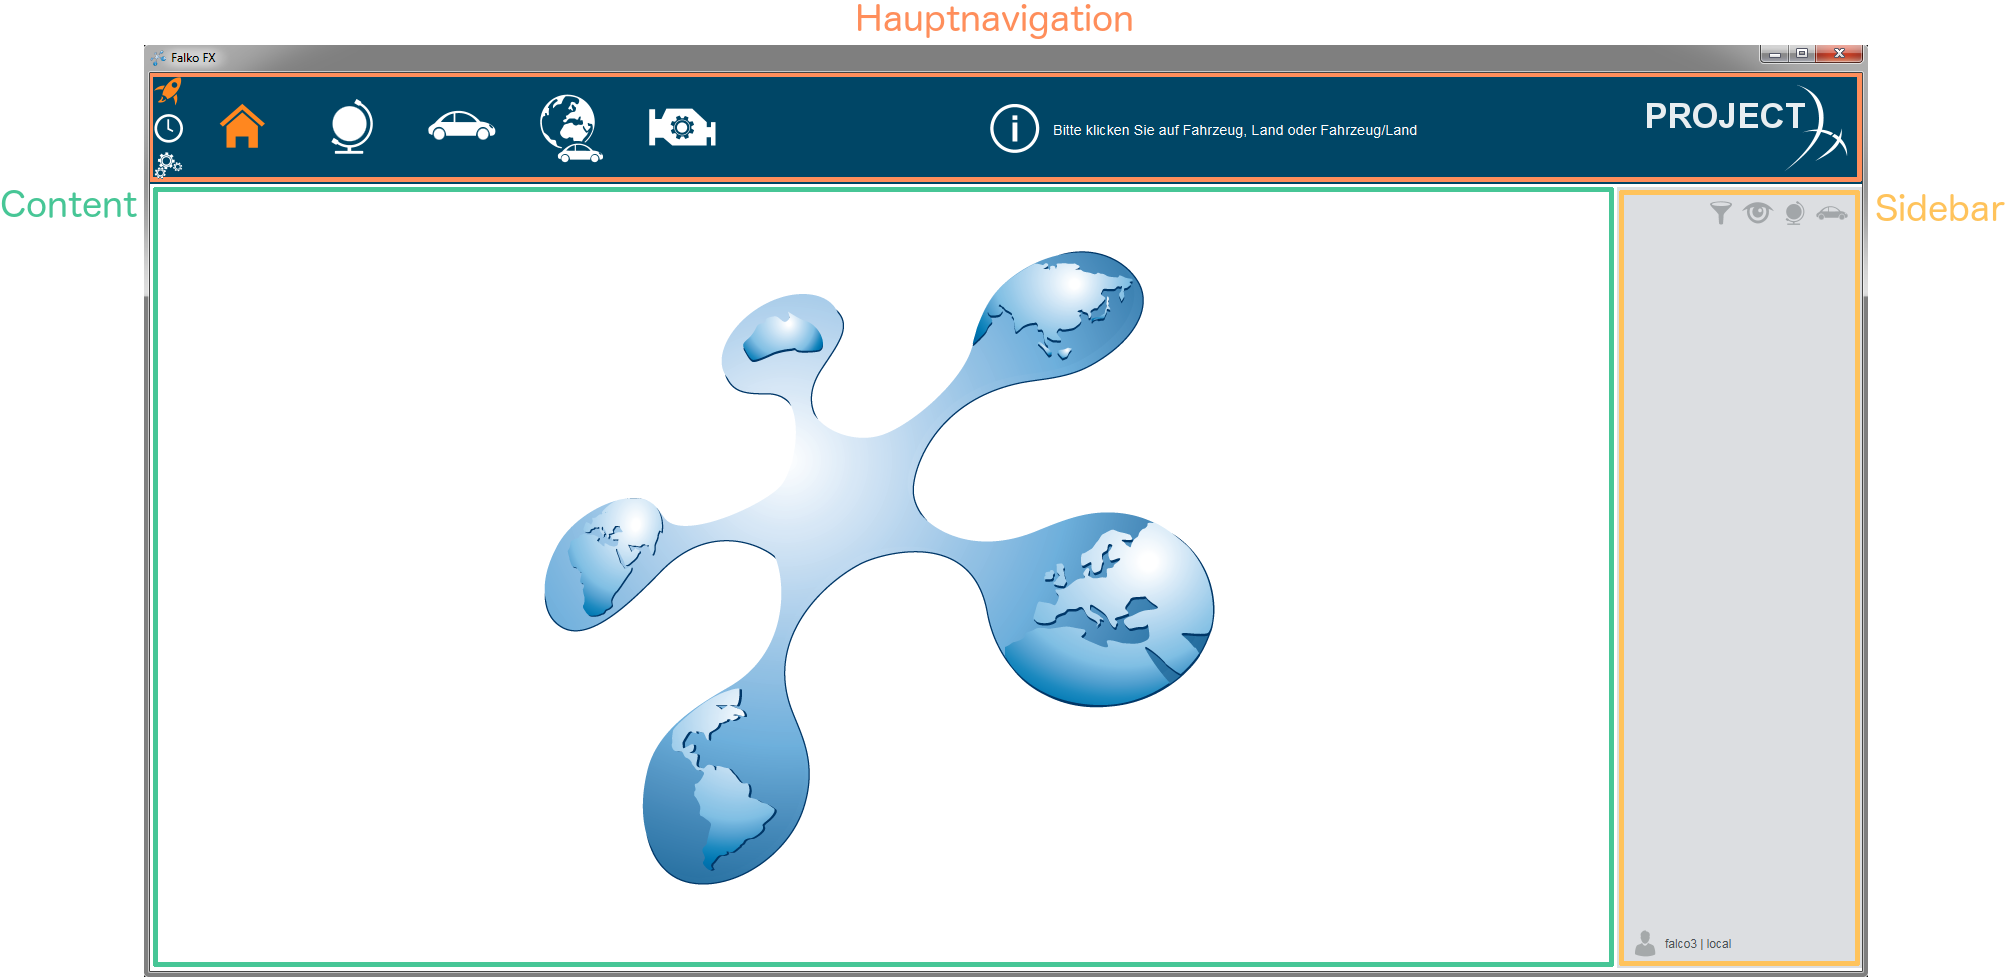
\includegraphics[width=0.8\textwidth]{grafiken/areas.png}
 \caption{Bereiche in FalkoFX}
 \label{fig:areas}
\end{figure}
Das Konzept der gemeinsamen Region wird hier durch die verschiedenen Hintergrundfarben realisiert und unterstreicht die unterschiedlichen Funktionalitäten.\par
\heading{Navigation}
Im Navigationsbereich findet sich im initialen Zustand die Hauptnavigation wieder. Durch die Bedienelemente an der linken Seite der Leiste kann zwischen folgenden Funktionen gewechselt werden:
\begin{enumerate}
	\item Hauptnavigation: Wechsel zwischen Standard-Anwendungsfällen und der verschiedenen Ansichten
	\item Versionsvergleich: Navigation für Anwendungsfälle mit Versionsvergleich (derzeit in Entwicklung)
	\item Einstellungen: Menü zum Ändern anwendungsspezifischer Einstellungen
\end{enumerate}
\begin{figure}[H]
 \centering
 
\includegraphics[width=0.05\textwidth]{grafiken/ribbon.png}
 \caption{Umschalten der Navigation}
 \label{fig:ribbon}
\end{figure}
Durch die vertikale Orientierung, der geringeren Größe und der Nähe zueinander heben sich die Elemente zum Umschalten der Navigation deutlich von den anderen Schaltflächen ab. Wird eines der Elemente angewählt, wird eine Aktion ausgeführt und die Kindelemente, falls vorhanden, werden mittels Animation sichtbar. Die nachfolgenden Elemente der höher liegenden Ebenen werden \enquote{zur Seite geschoben}.\par
\begin{figure}[H]
 \centering
 
\includegraphics[width=0.85\textwidth]{grafiken/navi.png}
 \caption{Navigationshierarchie}
 \label{fig:navi}
\end{figure}
Die Elemente einer einzigen Navigationsebene benötigen keine weitere Trennung. Durch den Freiraum zwischen diesen ist eine hinreichende Trennung erwirkt. Zwischen den verschiedenen Ebenen wird zusätzlich zu einer Farbabstufung eine weiße Trennlinie eingeblendet, die auf der linken Seite einen angedeuteten Pfeil enthält , der die Navigationshierarchie verdeutlicht. Dazu trägt ebenfalls die bereits erwähnte Animation bei.\par
Das Piktogramm des selektierten Navigationselementes wird orange eingefärbt, um die Orientierung zu gewährleisten. Kann der Nutzer eine bestimmte Interaktion nicht ausführen, erscheint das Icon grau.\par
Durch das Anklicken eines Icons wird der neue Bildschirm angezeigt. Dies geht oft mit dem Laden von Daten einher. Sollten Daten aus der Datenbank geladen werden müssen, wird währenddessen eine Ladeanimation angezeigt. Andernfalls wird der Bildschirm in weniger als 500 Millisekunden angezeigt, wodurch kein weiteres Feedback von Nöten ist. Im Gegenteil: Eine kurz aufblitzende Ladeanimation würde den Anwender eher irritieren als unterstützen.\par
Den Einstieg in jeden Anwendungsfall bietet der Filter. Der Filter besteht in der simpelsten Variante aus folgenden Komponenten:
\begin{itemize}
	\item \textbf{Radial-Menü:} Ein rundes Menü, in dem die zu filternden Attribute ausgewählt werden können
	\item \textbf{Multi-Level-Liste:} Eine mehrstufige Liste mit Suchfunktion, aus der Werte zu den Attributen angewählt werden können
	\item \textbf{Filterselektion:} Eine Liste, welche die aktuell ausgewählten Werte gruppiert darstellt und das Abwählen dieser Werte erlaubt
\end{itemize}
\begin{figure}[H]
 \centering
 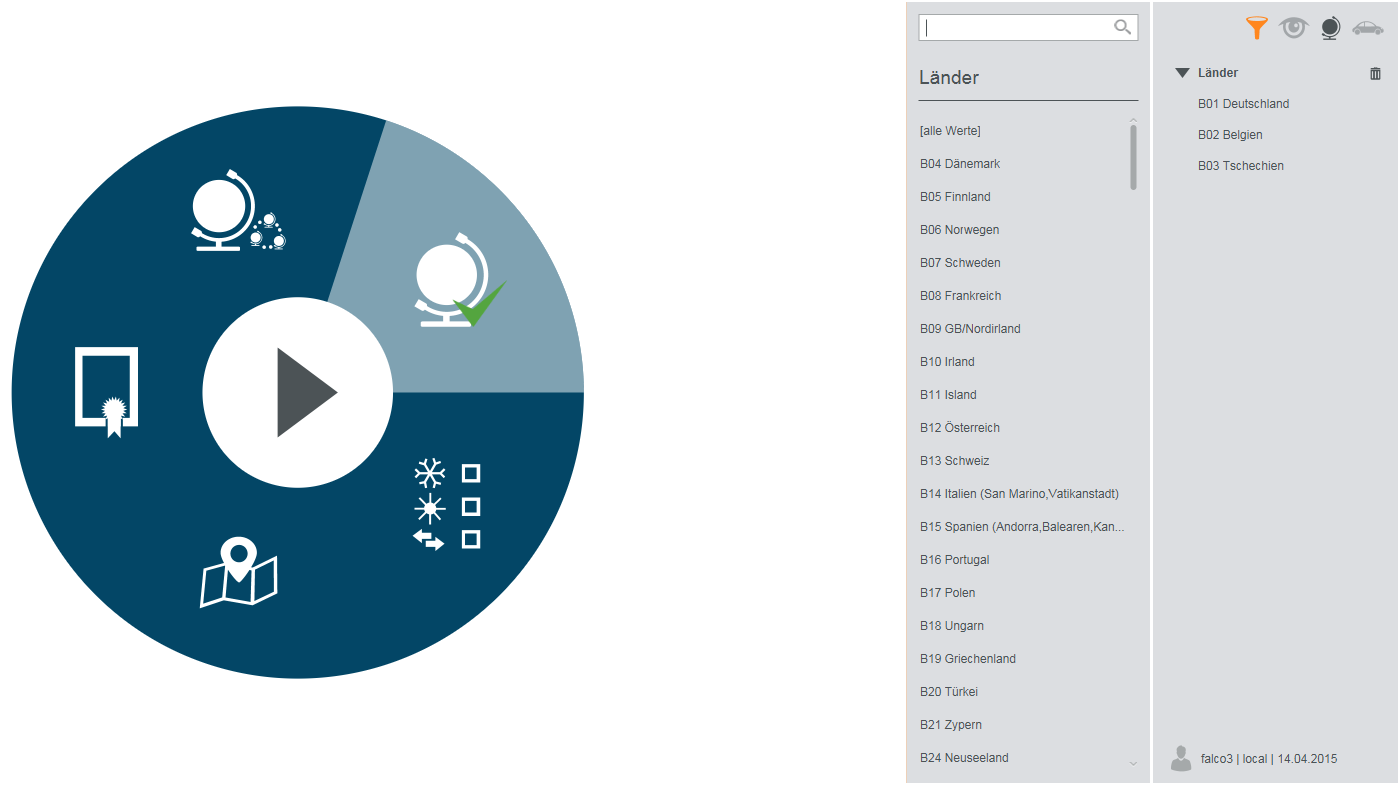
\includegraphics[width=0.6\textwidth]{grafiken/filter_short.png}
 \caption{Beispiel Filter}
 \label{fig:filter}
\end{figure}
Im Radial-Menü sind die Elemente kreisförmig um einen \textit{Play}-Button angeordnet, der standardmäßig deaktiviert ist. Erst, wenn die Ergebnismenge, die durch die gefilterten Attributwerte erzeugt wird, valide ist, wird der Button und das dazugehörige Navigationselement in der Navigationsleiste aktiviert. Die aktuelle Selektion in dem Menü wird durch einen helleren Kreisausschnitt über dem entsprechenden Element markiert. So wird dieser Bereich deutlich hervorgehoben.\par
Die Multi-Level-Liste enthält Werte, die als Filterkriterium ausgewählt werden können. Einige dieser Werte gruppieren weitere Werte und können nicht übernommen werden. Stattdessen öffnet sich beim Auswählen dieser Elemente eine untergeordnete Ebene der Multi-Level-Liste. Diese Werte sind mit einem Pfeil markiert, der in die gleiche Richtung zeigt, in die auch die nachfolgende Animation verläuft.\par
\begin{itemize}
	\item \textbf{Radial-Menü:} Ein rundes Menü, in dem die zu filternden Attribute ausgewählt werden können
	\item \textbf{Multi-Level-Liste:} Eine mehrstufige Liste mit Suchfunktion, aus der Werte zu den Attributen angewählt werden können
	\item \textbf{Filterselektion:} Eine Liste, welche die aktuell ausgewählten Werte gruppiert darstellt und das Abwählen dieser Werte erlaubt
\end{itemize}
\begin{figure}[H]
 \centering
 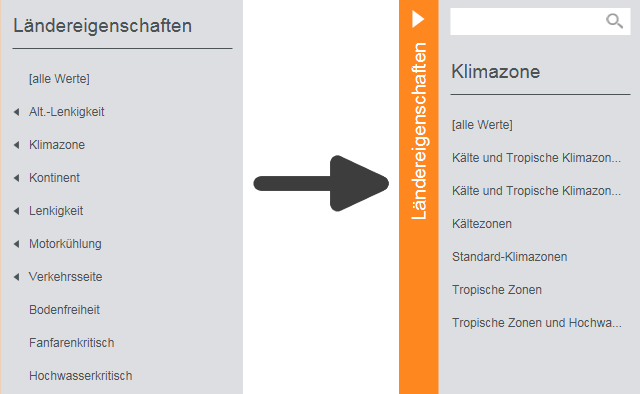
\includegraphics[width=0.4\textwidth]{grafiken/mll_combined.png}
 \caption{Multi-Level-Liste}
 \label{fig:mll}
\end{figure}
Nach dem Filtern der Daten lassen sich die Ergebnisansichten öffnen. Eine mögliche Präsentation ist die Tabellenansicht. Es handelt sich hierbei um eine komplexe Tabelle, die sämtliche Informationen darstellt. Die Spalten entsprechen den Attributen, zu denen erlaubte Werte im Filter ausgewählt wurden. Zusätzlich sind diese Attribute gruppiert. Die Trennung der Gruppen erfolgt durch deutlich sichtbare Linien, die vertikal zwischen den Spalten der einzelnen Gruppen verlaufen. Die einzelnen Gruppen lassen sich über Bedienelemente in der Sidebar aus- und einblenden, sowie per Drag\& Drop-Geste in der Reihenfolge vertauschen. Der um 45$^{\circ}$ geneigte Spaltenkopf sorgt für eine kompaktere Darstellung, da die minimale Spaltenbreite so nicht mehr durch den Titel der Spalte bestimmt wird. Besonders hilfreich ist diese Präsentation der Spaltenköpfe bei Werten, die nur sehr kurze Bezeichner annehmen. Der Beginn der gedrehten Beschriftungen ist dabei auf einer gedachten horizontalen Linie angeordnet. Auch in diesem Fall lässt sich das Gesetz der Kontinuität anwenden, wodurch die Überschriften als eine zusammengehörige Einheit wahrgenommen werden.\par
\begin{figure}[H]
 \centering
 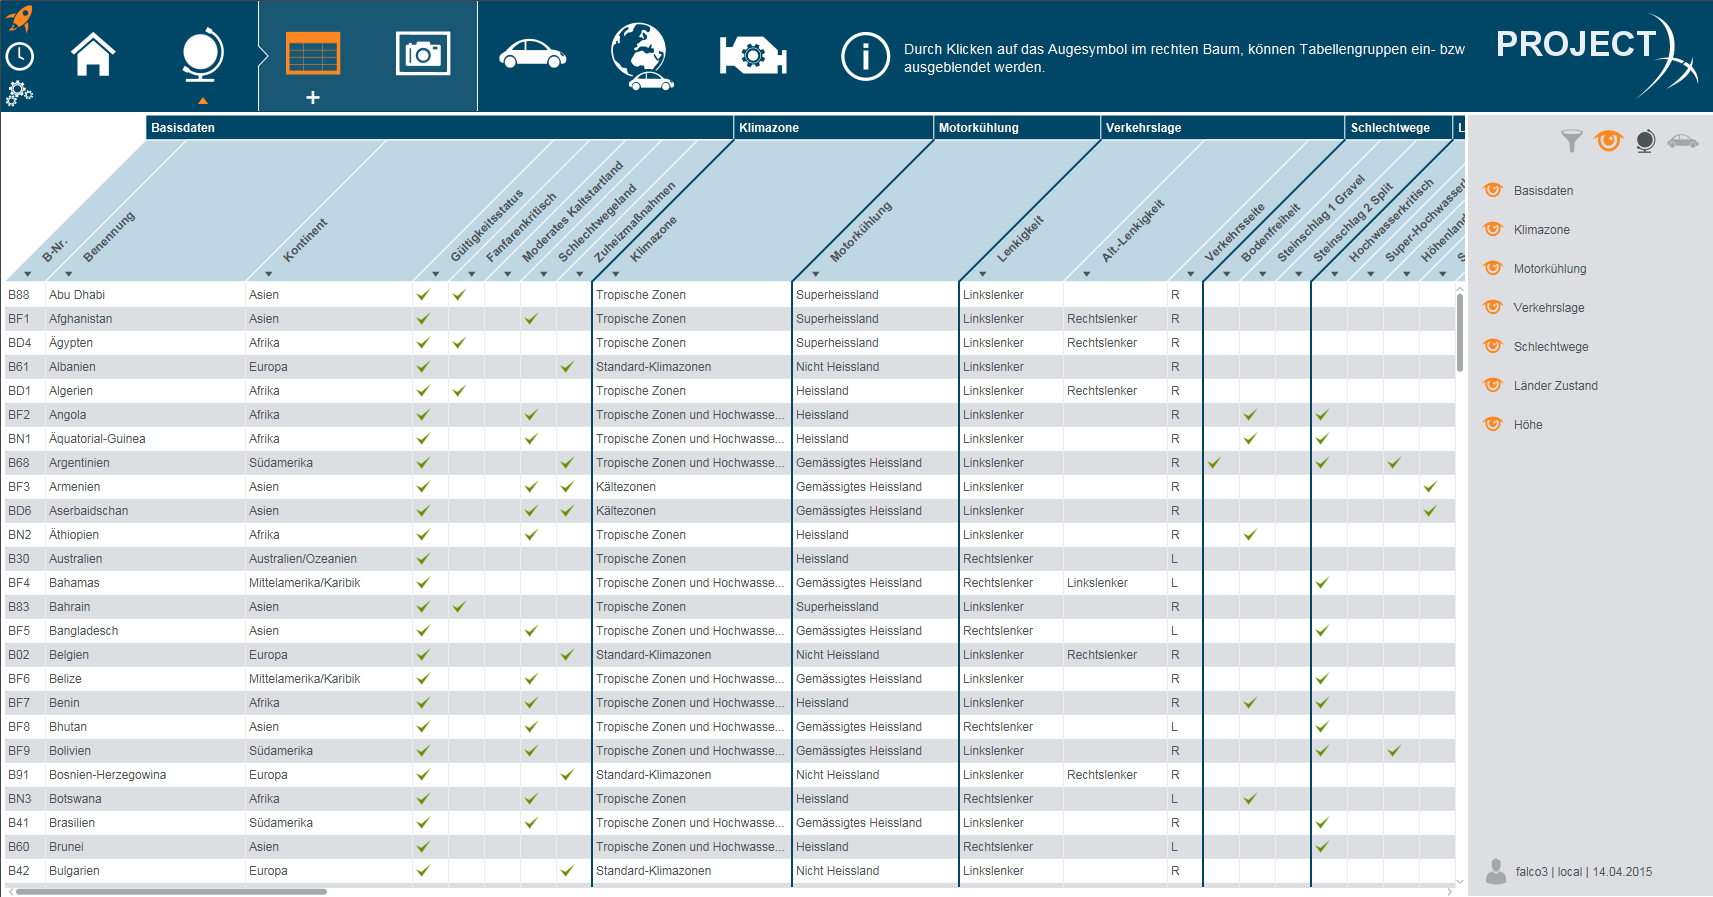
\includegraphics[width=0.6\textwidth]{grafiken/full_result_table.png}
 \caption{Ergebnistabelle}
 \label{fig:resultTable}
\end{figure}
Über die Pfeile im Spaltenkopf lässt sich ein \textit{Overlay} einblenden, in dem die präsentierten Daten auf einfache Weise zusätzlich eingeschränkt werden können, falls mit den aktuellen Einstellungen mehr Datensätze als gewünscht angezeigt werden. Zwar könnten die Pfeile als Elemente zur Umsortierung missverstanden werden, allerdings ist dies kein kritisches Problem, da sich das Overlay nach kurzer Zeit (oder nach dem Verlassen des Bereiches mit dem Mauscursor) schließt und andere Schaltflächen während der Anzeige nicht blockiert werden.\par
\begin{figure}[H]
 \centering
 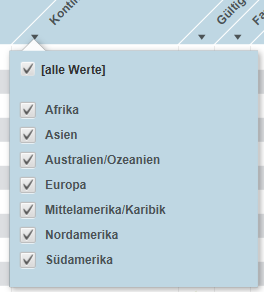
\includegraphics[width=0.3\textwidth]{grafiken/overlay.png}
 \caption{Schnellfilter-Overlay}
 \label{fig:autofilter}
\end{figure}
Im Navigationsbereich ist unter der Schaltfläche der Ergebnispräsentation ein zusätzliches Icon (\ding{58}) aufgetaucht. Bei Klick auf den Bereich des zusätzlichen Icons öffnet sich, mit einer \enquote{Aufklapp-} Animation ein untergeordnetes Menü, das erweiterte Optionen für die derzeit aktive Ansicht bereitstellt. Darunter fallen die Export-Möglichkeiten in PDF und Excel. Die Animation verdeutlicht die Zugehörigkeit zu dem Menüpunkt des aktuell ausgewählten Elements. Als ein mögliches Problem könnte sich das Auftauchen des Icons erweisen. Da der Menüpunkt schon vorher sichtbar war, wird die Änderung ggf. nicht wahrgenommen und ignoriert. Es wird also das Prinzip der Sichtbarkeit nicht vollständig erfüllt.\par
Eine weitere mögliche Ergebnispräsentation ist die Galerie. Hier werden im oberen Bereich Vorschaubilder für Daten angezeigt und darunter eine Detailansicht zum aktuell ausgewählten Element. Mit der Hilfe von $\blacktriangleright$ - und $\blacktriangleleft$ - Schaltflächen lassen sich die Objekte animiert durchschalten. Die aktuelle Selektion wird dadurch verdeutlicht, dass sich dass entsprechende Element stets mittig über der Detailansicht befindet. Zusätzlich wird ein Bezeichner in orangener Schrift darüber angezeigt und das Element wird durch Vergrößerung hervorgehoben. Alle anderen Elemente rücken durch eine geringe Opazität (\enquote{Deckkraft}) in den Hintergrund. Das Gesetz der Prägnanz wird hier durch mehrere ausschlaggebende Faktoren erfüllt und zeigt dem Anwender unmissverständlich die aktuelle Selektion an. \par
\begin{figure}[H]
 \centering
 \setlength{\fboxsep}{0pt}
 \setlength{\fboxrule}{0.5pt}
 \fbox{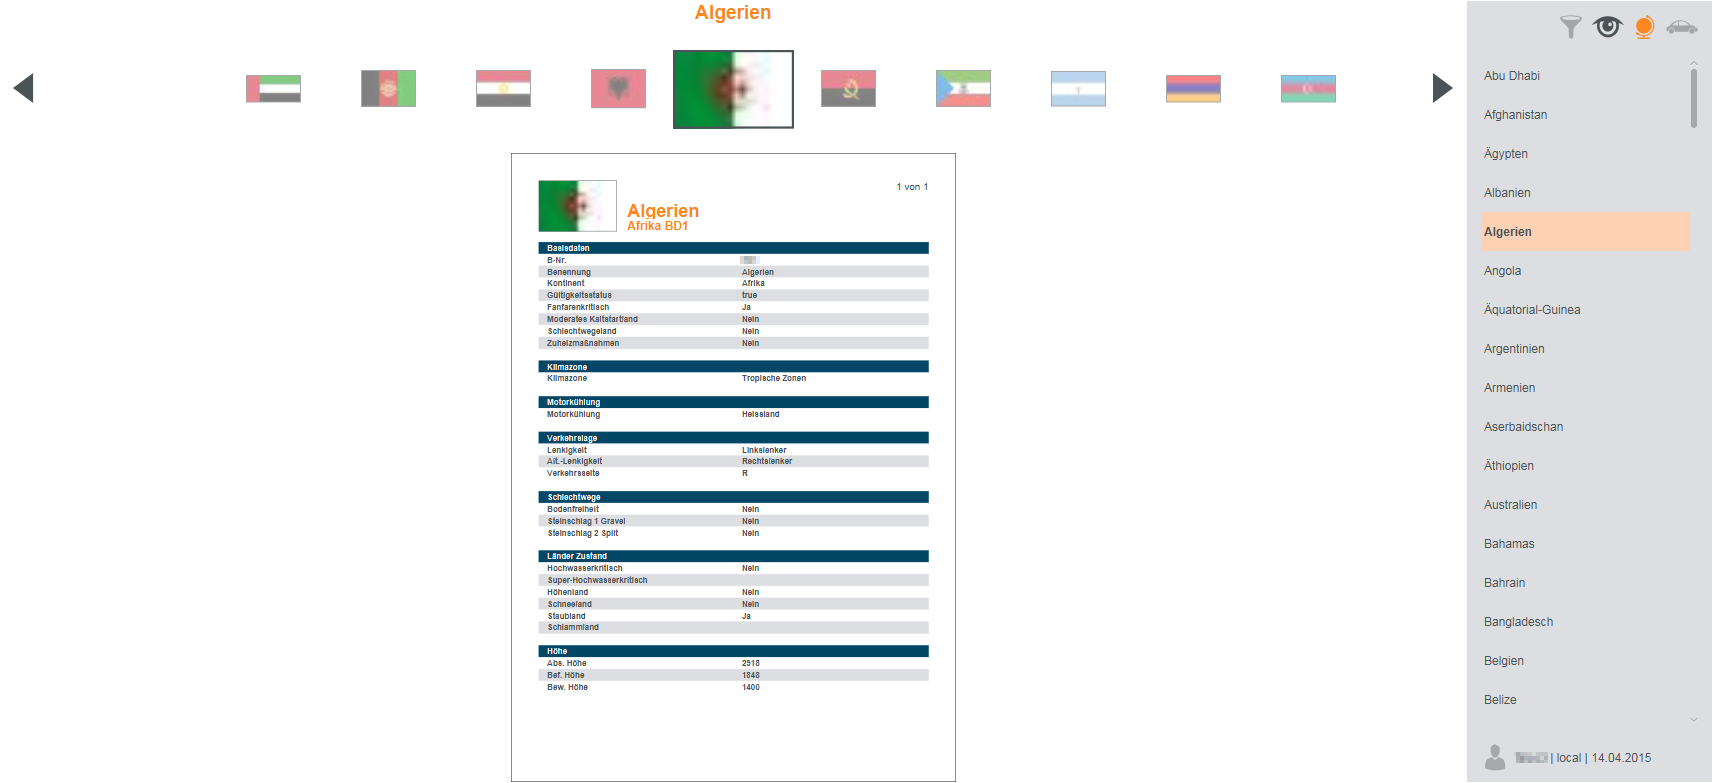
\includegraphics[width=0.6\textwidth]{grafiken/gallery.png}}
 \caption{Galerie}
 \label{fig:gallery}
\end{figure}
Für diese Ansicht ist in der Sidebar standardmäßig die \textit{Ergebnisvorschau} eingeblendet. Diese Ansicht bietet einen Überblick über alle Datensätze, die den Filterkriterien entsprechen. Die Selektion in dieser Liste ist mit der Selektion der Galerie-Komponente gekoppelt und wird so synchron gehalten. Auch die \textit{Ansichtskonfiguration}, die bereits aus der Tabellenansicht bekannt ist, kann hier angewählt und verändert werden. Daraufhin ändern sich die in der Detailansicht der Galerie dargestellten Attributgruppen.\par
Ein Klick auf die Detailansicht öffnet eine vergrößerte Darstellung, den sogenannten \textit{Lesemodus}. Er bietet die Möglichkeit, die zuvor dargestellten Informationen durch die größere Darstellung besser lesen zu können. Die vorherigen und Nachfolgenden Datensätze werden durch perspektivisch verschobene Seiten links und rechts der aktuell selektierten Seite eingeblendet. Durch Anklicken lassen sich diese, ebenfalls animiert, in den Vordergrund holen, während die aktive Seite \enquote{wegblättert}. Im Hintergrund verändert sich das selektierte Element in der Galerie. Durch das Anklicken des selbsterklärenden Tür-Icons in der unteren rechten Ecke lässt sich der Lesemodus wieder schließen.\par
\begin{figure}[H]
 \centering
 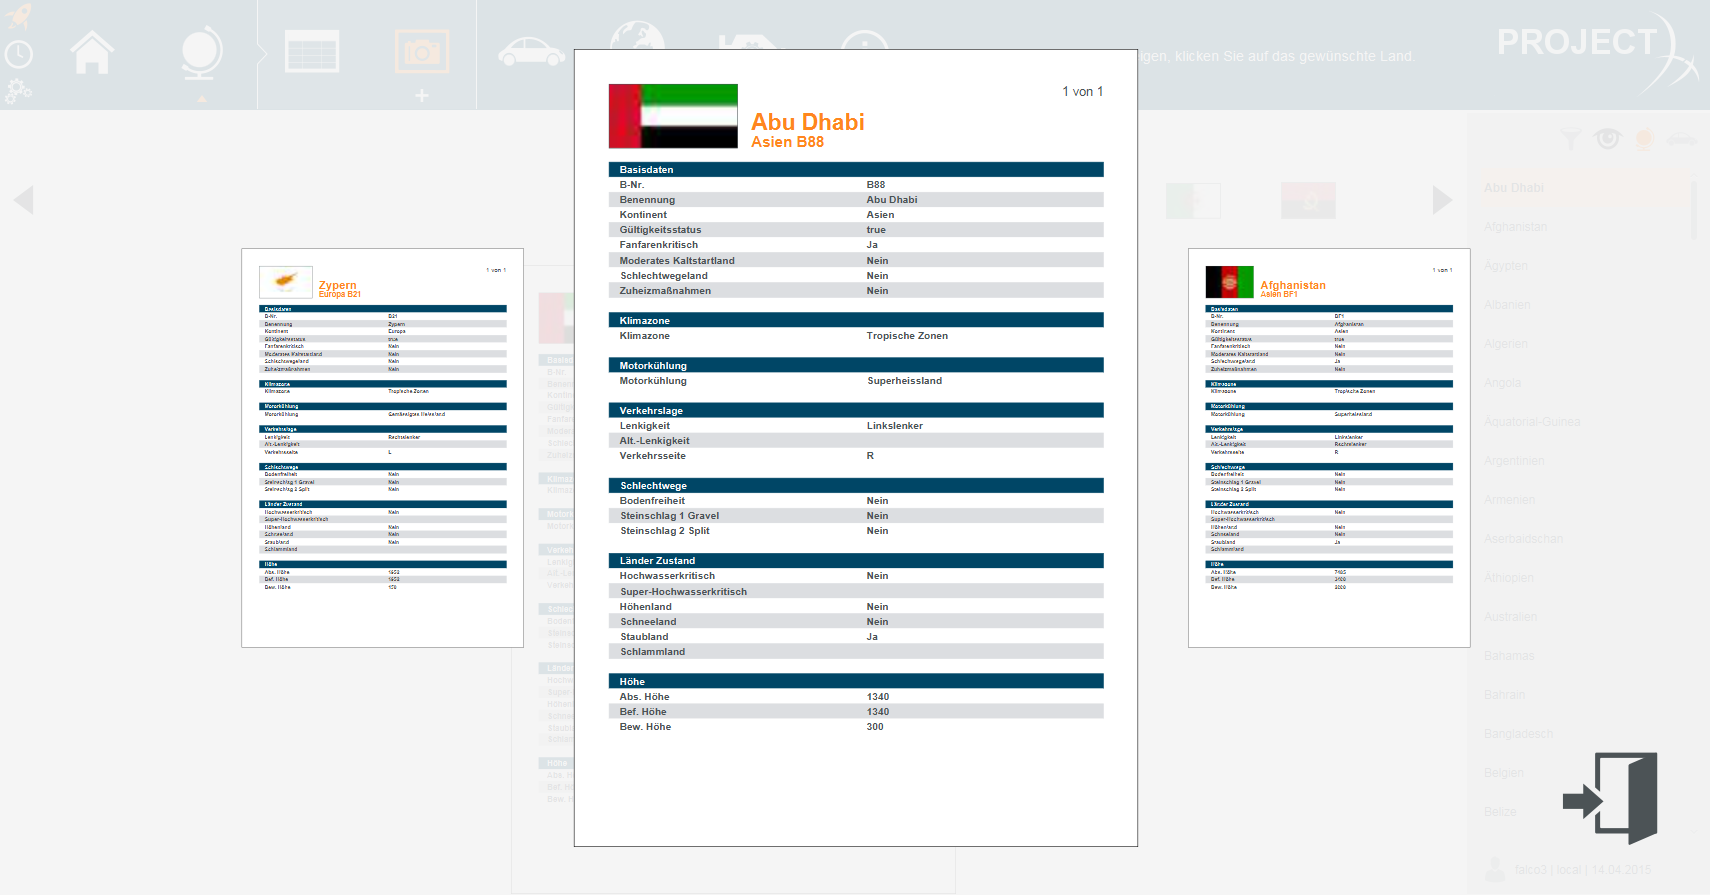
\includegraphics[width=0.6\textwidth]{grafiken/readmode.png}
 \caption{Lesemodus}
 \label{fig:readmode}
\end{figure}
Für den Anwendungsfall der Ländertypenübersicht (kurz: LTÜ) gibt es spezialisierte Filter- und Ergebnisansichten. Der Filter muss verschiedene Modelobjekte verwalten um die Daten der kombinierten Ergebnismenge anzeigen zu können. Daher existieren zwei unterschiedliche Filter-Menüs, die sich mittels Buttons umschalten lassen. Die Buttons sind so gestaltet, dass sie der schematischen Darstellung des RadialMenüs entsprechen und ein Piktogramm der zugrundeliegenden Objekttypen enthalten. So besitzen auch diese Elemente eine Selbsterklärungsfähigkeit.
\begin{figure}[H]
 \centering
 
\includegraphics[width=0.2\textwidth]{grafiken/filter_buttons.png}
 \caption{Filter umschalten}
 \label{fig:filterButtons}
\end{figure}
Die Ergebnispräsentation in diesem Anwendungsfall unterscheidet sich von der der anderen Anwendungsfälle. In der Ergebnistabelle werden die Daten in einer \textit{Matrixdarstellung} visualisiert. Die Zeilen werden zu Beginn mit den konfigurierbaren Informationen der Fahrzeugdaten befüllt. Danach werden weitere Spalten erstellt, die mit den einzelnen Ländern aus den gefilterten Länderdaten gekennzeichnet sind. Auf diese Weise ergibt sich eine Matrix aus Freigabedaten für jede mögliche Fahrzeug-Länder-Kombination. Durch die unterschiedliche Gestaltung des Spaltengruppenkopfes heben sich die Länderspalten von den Spalten mit den Fahrzeugattributen visuell ab und definieren so einen eigenen Abschnitt.
\begin{figure}[H]
 \centering
 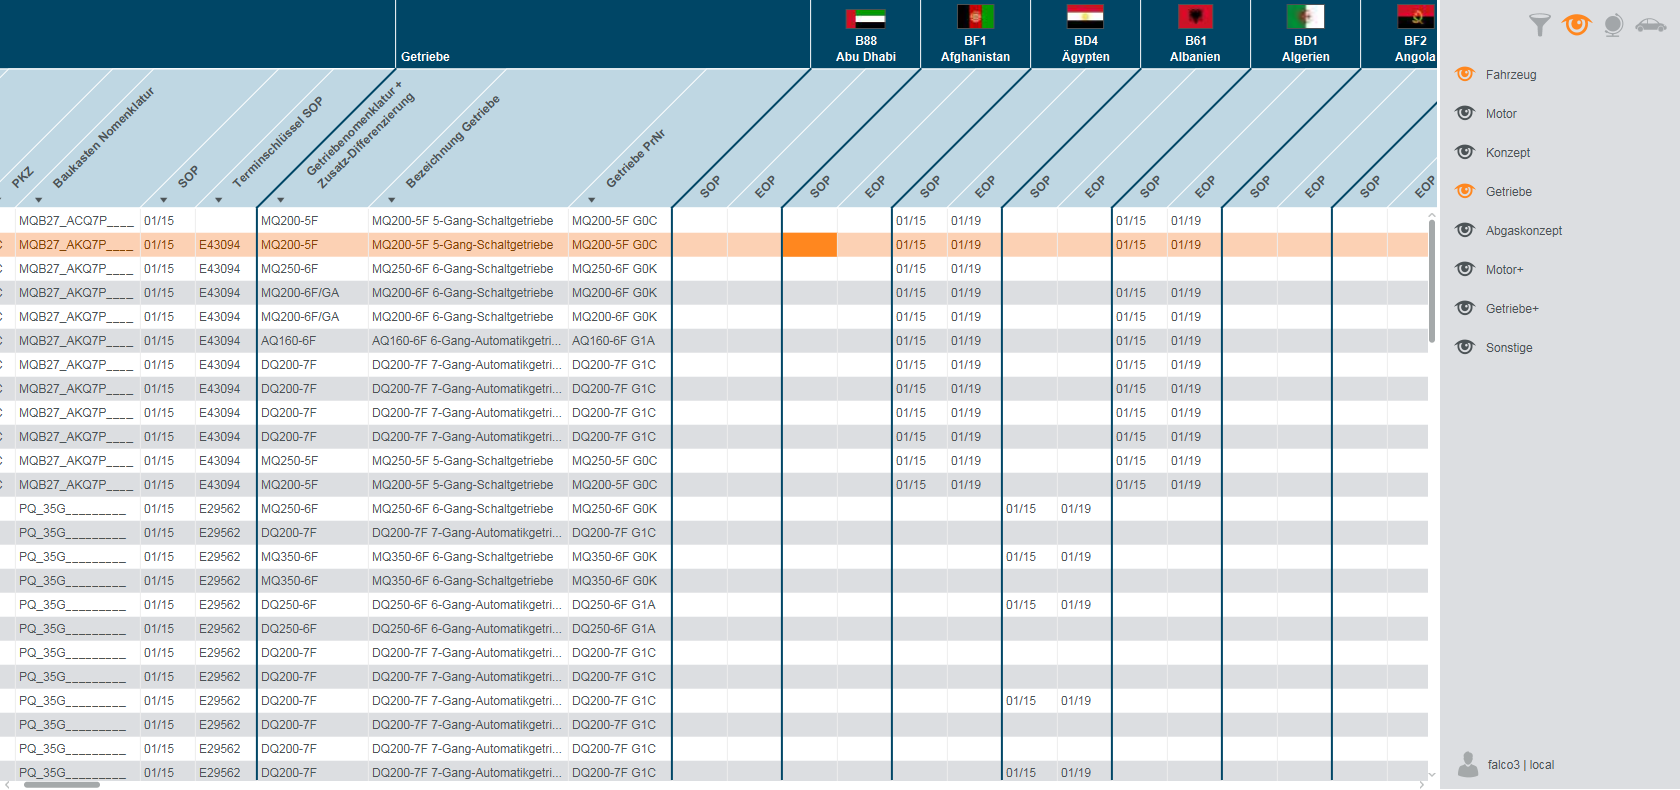
\includegraphics[width=0.6\textwidth]{grafiken/ltue_table.png}
 \caption{LTÜ Ergebnistabelle}
 \label{fig:ltueTable}
\end{figure}
Die Selektion findet zellenweise statt. Durch einen Doppelklick auf eine einzelne Freigaben können Details zu dieser Freigabe eingeblendet werden. Dennoch wird die Hintergrundfarbe der gesamten Zeile, in der sich die Selektion befindet, angepasst, damit die Orientierung in der komplexen Tabelle erleichtert wird.\par
Die Detailansicht zu einer Freigabe wird, anders als beim Lesemodus, nur im Content-Bereich der Applikation angezeigt. Hier wird für die Darstellung der Informationen weit weniger Platz benötigt, weshalb diese Darstellungsform ausreicht. Die Navigations- und die Seitenleiste sind weiterhin sichtbar, allerdings ist in der Sidebar keine Ansicht auswählbar und so wird diese leer angezeigt. Der Vorteil an der kontinuierlichen Sichtbarkeit der Navigationsleiste ist, dass der Kontext nicht verloren geht. Der Nutzer weiß also immer, wo er sich befindet, und welche Ansicht angezeigt wird, wenn er die Detailansicht wieder verlässt. Dies ist wichtig, da sowohl von der Tabellenansicht als auch von der Listenansicht, der weiteren verfügbaren Ergebnispräsentation, zu den Details einer Freigabe navigiert werden kann.\par
\begin{figure}[H]
 \centering
 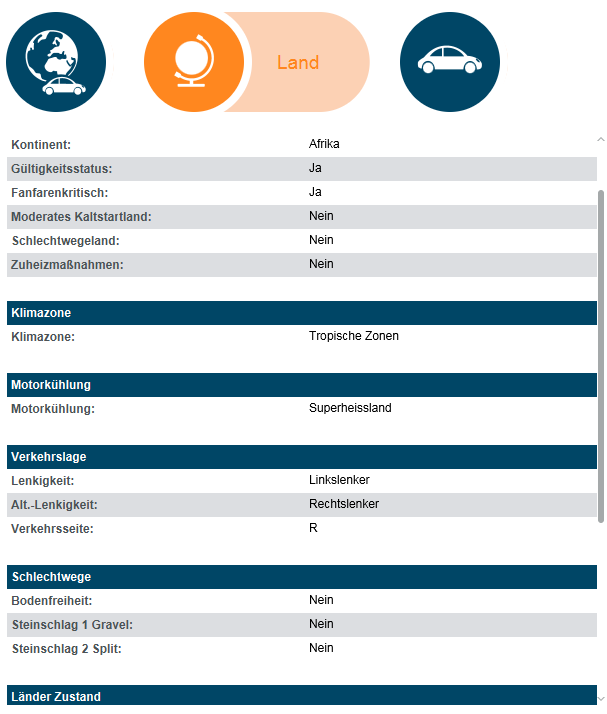
\includegraphics[width=0.3\textwidth]{grafiken/ltue_details.png}
 \caption{LTÜ Detailansicht}
 \label{fig:ltueDetails}
\end{figure}
Die Listenansicht ist eine zweigeteilte Darstellung. Auf der linken Seite befindet sich eine Tabelle mit den Fahrzeugen der Ergebnismenge als Inhalt. Auf der rechten Seite werden alle gefilterten Länder angezeigt, zu denen für das links ausgewählte Fahrzeug eine Freigabe existiert. Da der Inhalt der linken Tabelle deutlich umfangreicher ist, nimmt diese Seite deutlich mehr Platz ein als die Länderliste. Durch Doppelklick auf das entsprechende Land können die Details der Freigabe eingesehen werden.\par
\begin{figure}[H]
 \centering
 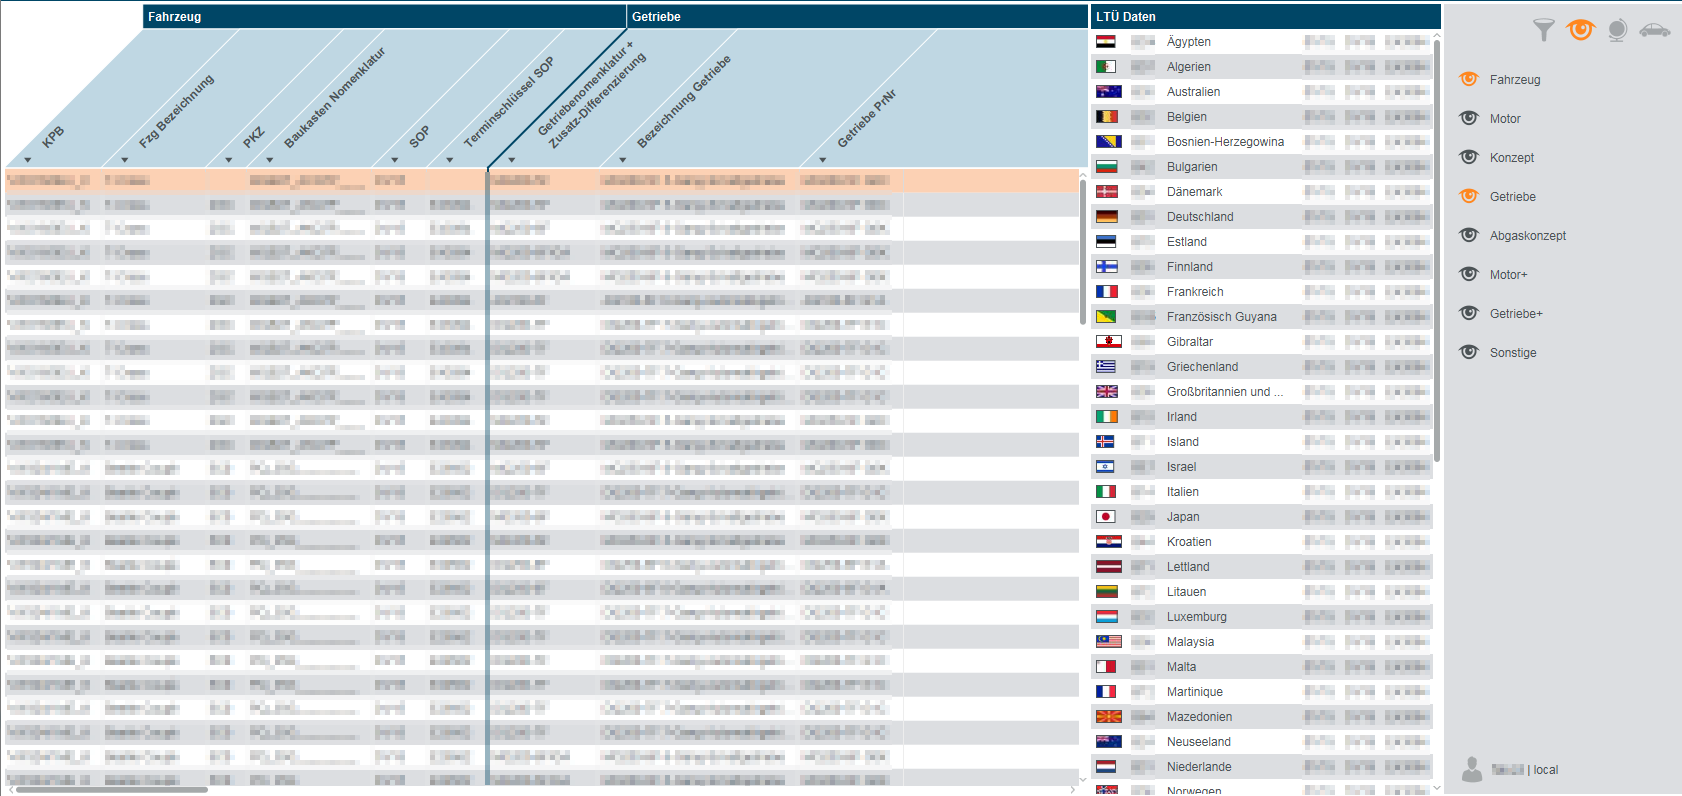
\includegraphics[width=0.6\textwidth]{grafiken/ltue_list.png}
 \caption{LTÜ Listenansicht}
 \label{fig:ltueList}
\end{figure}
Durch die Ähnlichkeit der beiden Komponenten wird die Zusammengehörigkeit schnell deutlich. Dieser Effekt wird zum einen durch die gleich gestalteten Zeilen erwirkt (Wechsel zwischen weißer und grauer Zeile) und zum anderen durch die aneinander ausgerichteten Kopfelemente. Dies sind der Spaltengruppenkopf der Tabelle und die \enquote{Überschrift} der Länderliste.\par
\subsection{Tastaturbedienbarkeit}
Die Anwendung ist momentan nur per Maus bedienbar. Die Möglichkeiten der Tastatur, die an jedem Arbeitsplatz zu finden ist, werden nicht ausgenutzt. Die Identifikation der Anwendungsbereiche, in denen die Tastatur eine alternative Bedienmöglichkeit darstellen kann, ist Ziel dieses Abschnittes. Dabei wird ein grundlegendes Konzept entworfen, für das in Abschnitt \ref{sec:designInteraction} spezialisierte Designlösungen gefunden werden.\par
Die erste Komponente, für die eine Tastatursteuerung denkbar wäre, ist die Navigation. Dabei sollten sowohl die Schaltflächen für das Umschalten der Navigationsleiste, als auch die Elemente per Tastatur bedienbar sein. So ist die grundlegende Steuerung der Anwendung möglich. Für die einzelnen Bildschirme müssen jeweils spezialisierte Lösungen gefunden werden.\par
Der erste Bildschirm, zu dem navigiert werden kann, ist der Filter. Hier gibt es das Radialmenü, die mehrstufige Liste und die Sidebar mit den gewählten Filterkriterien. Primär sollte die Liste mit der Tastatur bedient werden können, mit dem Ziel, Werte möglichst schnell zu finden und auszuwählen. Weiterführend kann die Steuerung für das Radialmenü umgesetzt werden, damit die Werte über verschiedene Attribute hinweg per Tastatur auswählbar sind. Die Bedienung der Sidebar ist eher nachrangig, da ihr Zweck ist, ausgewählte Werte wieder deselektieren zu können - folglich \enquote{nur} ein Mittel, um Fehler zu korrigieren.\par
In der Tabellenansicht, die in jedem Anwendungsfall verfügbar ist, ist eine Steuerung der Selektion denkbar. Außerdem sollte von einem Element zu den dazugehörigen Details gesprungen werden können, ohne dabei zur Maus wechseln zu müssen. Eine Steuerung der Sidebar wäre nur für den Reiter der Ansichtskonfiguration von Nöten, da die anderen verfügbaren Ansichten nur der Ergebnisvorschau dienen.\par
Ähnlich ist die Situation bei der Galerie. Auch hier wäre eine Tastatursteuerbarkeit der Selektion und das Öffnen der vergrößerten Ansicht im Lesemodus vorteilhaft. Das Durchschalten der Elemente kann ebenfalls mit der Tastatur erfolgen. Das Konzept dafür sollte nach Möglichkeit in allen Ergebnispräsentationen ähnlich sein. So sollte auch der Lesemodus nach dem gleichen Schema behandelt werden.\par
Die Listenansicht des LTÜ-Anwendungsfalles benötigt ebenfalls ein vergleichbares Konzept zur Steuerung. Die Schwierigkeit besteht darin, dass prinzipiell zwei Kontrollelemente gleichzeitig steuerbar sein müssen. Bei der Detailansicht, die von der Ergebnistabelle und der Listenansicht erreichbar ist, ist eine Unterstützung der Subnavigation in diesem Bildschirm denkbar.\par
\subsection{Übertragung von Touchgesten auf Maussteuerung}
Mit Blick auf den immer stärker werdenden Trend, auch Geschäftsanwendungen auf mobile Geräte zu portieren, soll an dieser Stelle geprüft werden, inwiefern die Touchgesten (vgl. Kapitel \ref{fig:touchGestures}) auf das Bedienkonzept am Desktop-PC übertragbar sind. Dies soll zum einen zu einer intuitiveren Bedienung mit der Maus beitragen und zum anderen für die Benutzung der Software auf sogenannten Convertibles vorsorgen. Convertibles sind Geräte, die sich als Laptop und Tablet gleichermaßen verwenden lassen.\par
Der Mauszeiger wird zu diesem Zweck als \enquote{Ersatz} für den Finger auf einem Touch-Display verwendet. Da es nur einen Mauszeiger und eine Maus gibt, ist es technisch gesehen nur möglich, Gesten durchzuführen, die genau einen Finger benötigen. Dies sind \textit{Tap}, \textit{Double Tap}, \textit{Drag}, \textit{Flick} und \textit{Press}. Die \textit{Tap} und \textit{Double Tap}-Gesten entsprechen sowohl von der Durchführung, als auch von der Semantik in der Regel dem einfachen Mausklick bzw. dem Doppelklick. Die \textit{Drag}-Geste ist der Drag\& Drop Aktion der Maus sehr ähnlich. An vielen Stellen jedoch, an denen bei mobilen Anwendungen \textit{Drag}-Gesten verwendet werden würden, wird die Benutzung eines UI-Elements auf dem Desktop-PC mit anderen Mitteln gelöst. Für den \textit{Flick}, auch \textit{Swipe} genannt, existiert kein Pendant im Pensum der normalen Maus- und Tastatur- Interaktion. Dennoch ist es denkbar, eine solche Geste mit einer schnell ausgeführten Drag\& Drop-Aktion zu ermöglichen. Auch der \textit{Press} kann mit den gegebenen Eingabemitteln umgesetzt werden. Eine solche Aktion ist jedoch in den meisten Fällen nur bedingt intuitiv verwendbar, da keine ähnlichen, dem Nutzer vertrauten, Aktionen für die Maussteuerung existieren. Als Ersatz kann der Rechtsklick bei der Desktop-Verwendung genutzt werden.\par
Die erste Komponente, für die eine Gesten-Unterstützung untersucht wird, ist die Navigationsleiste. Hier ist jedes aktive Element durch einen einfachen Mausklick verwendbar. Dieses Verhalten entspricht dem, was Nutzer mobiler Anwendungen bei der Bedienung erwarten würden. \textit{Swipe} oder \textit{Drag}- Gesten würden hier eher zu Verwirrung führen.\par
Die Bedienung des Radialmenüs im Filter ist zunächst nur mit einfachen Klicks auf die Zielelemente möglich. Als Alternative dazu sollten auch Touchgesten und deren Pendant auf Desktop-PCs bereitgestellt werden. Bei der Bedienung der Liste wird sich bislang auf das Scrollrad und den Scrollbalken verlassen. Auf Geräten, die nativ Toucheingaben unterstützen, ist das Scrolling per \textit{Drag} nativ bereits unterstützt. Um das Verhalten auf verschiedenen Plattformen anzugleichen und die Spanne von unterstützten Eingabemethoden zu erhöhen, sollte die Bedienmöglichkeit auch für die Maus umgesetzt werden. Durch diese Art von Scrolling kann vorallem in langen Listen genauer und zielgerichteter zu gesuchten Einträgen gelangt werden.\par %Sidebar?
In den Ergebnisansichten, in denen eine Tabelle bzw. eine Liste verwendet wird, stellt sich ein vergleichbares Problem. Jegliche Art von Tabelle oder Liste kann mit einer \textit{Drag}-Geste gescrollt werden, wenn die Eingabe über ein Touch-Display erfolgt. Die Steuerung sollte auch an diesen Stellen an die Touch- Bedienung angepasst werden. Dies sind im Speziellen die Ergebnistabelle und die Listenansicht.\par
In der Galerie muss die Umsetzung auf eine eigene Weise erfolgen. Die Leiste, in der die Vorschaubilder der angezeigten Datensätze angezeigt werden, kann ebenfalls mit neuen Bedienungsmöglichkeiten versehen werden, um die aktuelle Selektion zu verändern. Eine Steuerung, die nur über die Buttons links und rechts der Bordüre abgehandelt wird, schränkt den Nutzer stark ein. Ein ähnliches Verhalten zeigt der Lesemodus. Hier lässt sich das zentrierte, vergrößerte Datenblatt nur durch Anklicken eines der seitlichen Datenblätter ändern.\par
Zu guter Letzt existiert noch eine tabellenartige Komponente in der Detailansicht des LTÜ-Anwendungsfalles. Werden in der Komponente genügend Daten angezeigt, muss auch diese per Gesten gescrollt werden können.\par
\section{Design} \label{sec:designInteraction}
Nachdem die relevanten Stellen in der Analysephase aufgedeckt wurden, werden in diesem Abschnitt konzeptionelle Lösungen entwickelt, nach denen die Umsetzung erfolgen kann.\par
\subsection{Tastaturbedienung}
Das Implementieren der einzelnen Teillösungen ist nicht sinnvoll, ohne zunächst ein Gesamtkonzept entworfen zu haben. Wie in der Analysephase festgestellt, gibt es mehrere Komponenten, für die eine Tastaturbedienung ermöglicht werden soll. Einige dieser Komponenten können zeitgleich auf dem Bildschirm sichtbar sein (z.B. die Navigationsleiste und die mehrstufige Liste der Filteransicht). Das führt in der Bedienung zu Konflikten, da Tastatureingaben, nach dem in Abschnitt \ref{sec:javafxEventhandling} beschriebenen Event-Handling-Konzept, nur an einem spezifischen Knoten im Szenegraphen angelangen, wenn dieser den Eingabefokus besitzt. Es ist demnach nicht möglich, die Events an einem bestimmten Knoten zu behandeln indem der Fokus auf dieses Element gesetzt wird. Das Problem kann jedoch umgangen werden. Anstatt EventHandler an den jeweiligen Komponenten zu registrieren, können die EventHandler direkt an dem \textit{Szene}-Knoten, also der Wurzel des Szenegraphen, angemeldet werden.\par
\heading{Sekundäre Funktionalitäten}
Ein Konzept, das in modernen Anwendungen oft Verwendung findet sind die \textit{Mnemonics}. Mnemonics sind Tastenkombinationen mit denen in der Regel sekundäre Funktionen, wie zum Beispiel Menüs, bedient werden können. Eine Methode, die in modernen Anwendungen Verwendung findet ist das einmalige Drücken der \textit{Alt}-Taste, das die Einblendung der möglichen Tastenkombinationen zufolge hat. Eine ähnliche Umsetzung kann für die Sekundärfunktionen von FalkoFX erfolgen. Dazu zählen vorallem die Navigationsleiste und die Sidebar. Um den Nutzer dabei zu unterstützen, die mit Mnemonics versehenen Elemente zu identifizieren, wird über der gesamten Anwendung eine leicht transparente Komponente eingeblendet, die genau die Stellen ausspart, an denen sich steuerbare Objekte befinden. Zudem wird in den dadurch erzeugten Bereichen die Tastenkombination eingeblendet, welche die entsprechende Aktion ausführt.\par
Für das Steuern der Navigationsleiste eignen sich die Zahlentasten am besten. Die verschiedenen Navigationsleisten werden parallel dazu mit den Funktionstasten F1, F2, etc. umgeschaltet. Um die Sidebar zu bedienen sollten im Optimalfall sprechende Kombinationen gewählt werden. Das wäre beispielsweise der Buchstabe \enquote{E} für Ergebniskonfiguration oder \enquote{F} für die Filterauswahl. Generell gilt: Es sollten nur die Elemente mit Mnemonics versehen werden, die sichtbar, aktiv und auch mit normalen Mausklicks zu verwenden sind.\par
Die Haupteingabe findet immer in dem derzeit im Content-Bereich aktiven Bildschirm statt.

\subsection{Gestensteuerung}
\section{Implementierung} \label{sec:interactionImplementation}
